\باب{فوریئر تسلسل}
انجینئری مسائل میں دوری تفاعل عموماً پائے جاتے ہیں جن کو سادہ دوری تفاعل مثلاً \عددی{\sin} اور \عددی{\cos} کی روپ میں لکھنا مفید ثابت ہوتا ہے۔اسی عمل سے فوریئر تسلسل\حاشیہد{فرانسیسی ریاضی دان اور ماہر طبیعیات جین بپٹسٹ یوسف فوریئر [1768-1830]} ابھر کر سامنے آتی ہے جو سادہ تفرقی مساوات اور جزوی تفرقی مساوات کے حل میں کلیدی کردار ادا کرتی ہے۔

فوریئر تسلسل کا نظریہ پیچیدہ ہے جبکہ اس کا استعمال نہایت آسان  ہے۔چونکہ بہت سارے غیر استمراری تفاعل کا فوریئر تسلسل حاصل کرنا ممکن ہے جبکہ ان کا ٹیلر تسلسل نہیں پایا جاتا ہے لہٰذا فوریئر تسلسل کو ٹیلر تسلسل کی عالمگیر صورت تصور کیا جا سکتا ہے۔

اس باب میں فوریئر تسلسل سے وابستہ تصورات، حقائق اور تکنیکی تراکیب پر غور کیا جائے گا۔اس کے علاوہ ان کی استعمال پر غور کیا جائے گا۔اگلے باب میں جزوی تفرقی مساوات کی حل میں ان کا استعمال دکھایا جائے گا۔

اس باب کی آخری حصے میں فوریئر تکمل پر غور کیا جائے گا جنہیں اگلے باب میں جزوی تفرقی مساوات کی حل میں استعمال کیا جائے گا۔

\حصہ{دوری تفاعل، تکونیاتی تسلسل}
تفاعل \عددی{f(x)} اس صورت \اصطلاح{دوری}\فرہنگ{دوری}\حاشیہب{periodic}\فرہنگ{periodic} کہلاتا ہے کہ جب پورے حقیقی \عددی{x} پر \عددی{f(x)} معین ہو اور ایسا مثبت عدد \عددی{T} پایا جاتا ہو کہ تمام \عددی{x} پر درج ذیل درست ہو۔
\begin{align}\label{مساوات_فوریئر_دوری_تعریف_الف}
f(x+T)=f(x)\quad \quad \quad \text{\RL{تمام $x$ کے لئے}}
\end{align} 
عددی \عددی{T} کو \عددی{f(x)} کا \اصطلاح{دوری عرصہ}\فرہنگ{دوری عرصہ}\حاشیہب{period}\فرہنگ{period} کہتے\حاشیہد{تفاعل \عددی{f(x)} کا کم تر دوری عرصہ  \عددی{T (>0)}، اگر موجود ہو، \عددی{f(x)} کا اوّلی دوری عرصہ کہلاتا ہے۔مثلاً \عددی{\sin x} اور \عددی{\sin 2x} کا بالترتیب اوّلی دوری عرصہ \عددی{2\pi} اور \عددی{\pi} ہے جبکہ \عددی{f=\text{مستقل}} کا کوئی دوری عرصہ نہیں پایا جاتا ہے۔} ہیں۔\عددی{T} کے برابر  \عددی{f(x)} کے کسی بھی وقفے کا ترسیم دہراتے ہوئے ایسے تفاعل کا ترسیم حاصل کیا جاتا ہے (شکل \حوالہ{شکل_فوریئر_دوری_تفاعل})۔عملی استعمال میں عموماً  دوری اعمال اور تفاعل  پائے جاتے ہیں۔
\begin{figure}
\centering
\begin{tikzpicture}
\draw(-3,0)--(5,0)node[right]{$x$};
\draw(0,-1.2)--(0,1.2)node[left]{$f(x)$};
\draw[domain=-400:850,samples=100] plot ({\x/200},{0.5*sin(\x)-0.5/2*sin(2*\x)});
\draw(237/200,-0.6)--++(0,-0.3)coordinate[pos=0.75](kA);
\draw(237/200+360/200,-0.6)--++(0,-0.3)coordinate[pos=0.75](kB);
\draw[stealth-stealth] (kA)--(kB)node[pos=0.5,fill=white]{$T$};
\end{tikzpicture}
\caption{دوری تفاعل}
\label{شکل_فوریئر_دوری_تفاعل}
\end{figure} 

دوری تفاعل کی مثالیں \عددی{\sin x} اور \عددی{\cos x} ہیں۔اس کے علاوہ \عددی{f=c=\text{مستقل}} بھی دوری تفاعل کی تعریف (مساوات \حوالہ{مساوات_فوریئر_دوری_تعریف_الف} پر ہر مثبت \عددی{T} کے لئے) پورا اترنے کی بنا  دوری تفاعل ہے۔

مساوات \حوالہ{مساوات_فوریئر_دوری_تعریف_الف} سے ظاہر ہے کہ عدد صحیح \عددی{n} کی صورت میں درج ذیل ہو گا۔
\begin{align*}
f(x+nT)=f(x)\quad \quad \quad \text{\RL{تمام $x$ کے لئے}}
\end{align*}
یوں \عددی{2T}، \عددی{3T}، \عددی{4T}، \نقطے بھی تفاعل \عددی{f(x)} کے دوری عرصے ہیں۔مزید اگر تفاعل \عددی{f(x)} کا اور \عددی{g(x)} کا دوری عرصہ \عددی{T} ہو تب درج ذیل تفاعل
\begin{align*}
h(x)=af(x)+bg(x)\quad \quad \text{\RL{مستقل $a$، $b$}}
\end{align*}
 کا دوری عرصہ بھی \عددی{T} ہو گا جہاں \عددی{a} اور \عددی{b} مستقل ہیں۔

اس باب کی شروع میں ہم ایسے مختلف تفاعل جن کا دوری عرصہ \عددی{2\pi} ہو کو درج ذیل سادہ تفاعل کی  روپ میں ظاہر کرنا سیکھیں گے
\begin{align*}
1,\quad \cos x,\, \sin x,\quad \cos 2x,\, \sin 2x,\,\cdots, \quad \cos nx,\, \sin nx,\,\cdots
\end{align*}
جن کا دوری عرصہ \عددی{2\pi} ہے (شکل \حوالہ{شکل_فوریئر_سائن_کوسائن_یکساں_دوری_عرصہ})۔ہم دیکھیں گے کہ  ایسا کرتے ہوئے درج ذیل طرز کی تسلسل حاصل ہو گی
\begin{align}\label{مساوات_فوریئر_دوری_تعریف_ب}
a_0+a_1\cos x+b_1\sin x+a_2\cos 2x+b_2\sin 2x+\cdots
\end{align}
جہاں \عددی{a_0}، \عددی{a_1}، \عددی{a_2}،\نقطے، \عددی{b_1}،\عددی{b_2}،\نقطے حقیقی مستقل ہوں گے۔اس تسلسل کو \اصطلاح{تکونیاتی تسلسل}\فرہنگ{تسلسل!تکونیاتی}\حاشیہب{trigonometric series}\فرہنگ{series!trigonometric} کہتے ہیں جبکہ \عددی{a_n} اور \عددی{b_n} تسلسل کی \اصطلاح{عددی سر}\فرہنگ{عددی سر}\حاشیہب{coefficients}\فرہنگ{coefficients} کہلاتے ہیں۔چونکہ اس تسلسل کے ہر رکن کا دوری عرصہ \عددی{2\pi} ہے لہٰذا اگر یہ تسلسل مرکوز ہو تب یہ ایسا تفاعل ہو گا جس کا دوری عرصہ \عددی{2\pi} ہو گا۔
 
\begin{figure}
\centering
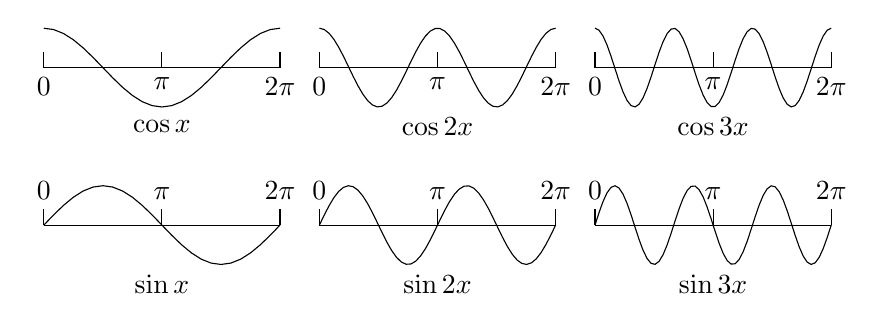
\begin{tikzpicture}
\pgfmathsetmacro{\amp}{0.5}
\pgfmathsetmacro{\pp}{120}
%
\draw(0,0)--(360/\pp,0);
\foreach \x/\l in {0/0,1.5/\pi,3/2\pi}{\draw(\x,0)node[below]{$\l$}--++(0,0.2);}
\draw[domain=0:360] plot ({\x/\pp},{\amp*cos(\x)});
\draw(1.5,-1.5*\amp)node{$\cos x$};
%
\begin{scope}[shift={(0,-4*\amp)}]
\draw(0,0)--(360/\pp,0);
\foreach \x/\l in {0/0,1.5/\pi,3/2\pi}{\draw(\x,0)--++(0,0.2)node[above]{$\l$};}
\draw[domain=0:360] plot ({\x/\pp},{\amp*sin(\x)});
\draw(1.5,-1.5*\amp)node{$\sin x$};
\end{scope}
%===========================
\begin{scope}[shift={(3.5,0)}]
\draw(0,0)--(360/\pp,0);
\foreach \x/\l in {0/0,1.5/\pi,3/2\pi}{\draw(\x,0)node[below]{$\l$}--++(0,0.2);}
\draw[domain=0:360,samples=50] plot ({\x/\pp},{\amp*cos(2*\x)});
\draw(1.5,-1.5*\amp)node{$\cos 2x$};
%
\begin{scope}[shift={(0,-4*\amp)}]
\draw(0,0)--(360/\pp,0);
\foreach \x/\l in {0/0,1.5/\pi,3/2\pi}{\draw(\x,0)--++(0,0.2)node[above]{$\l$};}
\draw[domain=0:360,samples=50] plot ({\x/\pp},{\amp*sin(2*\x)});
\draw(1.5,-1.5*\amp)node{$\sin 2x$};
\end{scope}
\end{scope}
%================================
\begin{scope}[shift={(7,0)}]
\draw(0,0)--(360/\pp,0);
\foreach \x/\l in {0/0,1.5/\pi,3/2\pi}{\draw(\x,0)node[below]{$\l$}--++(0,0.2);}
\draw[domain=0:360,samples=60] plot ({\x/\pp},{\amp*cos(3*\x)});
\draw(1.5,-1.5*\amp)node{$\cos 3x$};
%
\begin{scope}[shift={(0,-4*\amp)}]
\draw(0,0)--(360/\pp,0);
\foreach \x/\l in {0/0,1.5/\pi,3/2\pi}{\draw(\x,0)--++(0,0.2)node[above]{$\l$};}
\draw[domain=0:360,samples=60] plot ({\x/\pp},{\amp*sin(3*\x)});
\draw(1.5,-1.5*\amp)node{$\sin 3x$};
\end{scope}
\end{scope}
\end{tikzpicture}
\caption{سائن اور کوسائن تفاعل جن کا دوری عرصہ $2\pi$ ہے}
\label{شکل_فوریئر_سائن_کوسائن_یکساں_دوری_عرصہ}
\end{figure}

انجینئری میں واقع تفاعل پیچیدہ  ہوتے ہیں جنہیں سادہ دوری تفاعل کی روپ میں لکھنا مدد گار ثابت ہوتا ہے۔ہم دیکھیں گے کہ عملی استعمال، مثلاً ارتعاش، میں پائے جانے والا  تقریباً ہر دوری تفاعل \عددی{f(x)} جس کا دوری عرصہ \عددی{2\pi} ہو  کو فوریئر تسلسل کی روپ میں لکھنا ممکن ہو گا۔ہم مساوات \حوالہ{مساوات_فوریئر_دوری_تعریف_ب} کے عددی سر حاصل کرنے کے ایسے کلیات دریافت کریں گے جو \عددی{f(x)} پر منحصر ہوں گے اور جنہیں استعمال کرتے ہوئے حاصل تسلسل مرکوز ہو گا جس کا مجموعہ \عددی{f(x)} کے برابر ہو گا۔اس کے بعد ہم حاصل کلیات کو عمومی شکل دیتے ہوئے ان  کو کسی بھی دوری عرصہ کے تفاعل کے لئے قابل استعمال بنائیں گے۔ایسا کرنا نہایت آسان ثابت ہو گا۔

%============================
\حصہء{سوالات}

%===================
\ابتدا{سوال}\شناخت{سوال_فوریئر_کمتر_دوری_عرصہ_الف}\quad دیے گئے تفاعل کا کم تر دوری عرصہ دریافت کریں۔
\begin{align*}
\cos x,\, \sin x,\, \cos 2x,\, \sin 2x,\, \cos \pi x,\, \sin \pi x,\, \cos 2\pi x,\, \sin 2\pi x
\end{align*}
جوابات:\quad
$2\pi, 2\pi,\pi, \pi,2,2,1,1$

\انتہا{سوال}
%======================
\ابتدا{سوال}\quad اگر تفاعل \عددی{f(x)} کا دوری عرصہ \عددی{T} ہو تب ثابت کریں کہ \عددی{nT} جہاں \عددی{n=2,3,\cdots} ہے بھی اس تفاعل کا دوری عرصہ ہو گا۔
\انتہا{سوال}
%=====================
\ابتدا{سوال}\quad ثابت کریں کہ اگر تفاعل \عددی{f(x)} کا  اور تفاعل \عددی{g(x)} کا دوری عرصہ \عددی{T} ہو تب تفاعل \عددی{h(x)=af(x)+bg(x)} کا دوری عرصہ بھی \عددی{T} ہو گا، جہاں \عددی{a} اور \عددی{b} مستقل ہیں۔یوں دوری عرصہ \عددی{T} رکھنے والے تمام تفاعل سمتی فضا پیدا کرتے ہیں۔
\انتہا{سوال}
%=====================
\ابتدا{سوال}\quad ثابت کریں کہ تفاعل \عددی{f(x)=\text{مستقل}} ایسا دوری تفاعل ہے جس کا دوری عرصہ \عددی{T} کوئی بھی مثبت عدد ہو سکتا ہے۔
\انتہا{سوال}
%========================
\ابتدا{سوال}\quad ثابت کریں کہ  تفاعل \عددی{f(x)} کا دوری عرصہ \عددی{T} ہونے کی صورت میں \عددی{x} کے دوری تفاعل  \عددی{f(ax), a\ne 0} کا دوری عرصہ \عددی{\tfrac{T}{a}} ہو گا جبکہ \عددی{x} کے دوری  تفاعل \عددی{f(\tfrac{x}{b}), b\ne 0}  کا دوری عرصہ \عددی{bT} ہو گا۔ان نتائج کی تصدیق \عددی{f(x)=\cos x,\, a=b=2} کے لئے کریں۔ 
\انتہا{سوال}
%========================
سوال \حوالہ{سوال_فوریئر_ترسیم_کھینچیں_الف} تا سوال \حوالہ{سوال_فوریئر_ترسیم_کھینچیں_ب} میں دیے گئے تفاعل کا ترسیم کھینچیں۔

%===============
\ابتدا{سوال}\شناخت{سوال_فوریئر_ترسیم_کھینچیں_الف}\quad
$\sin x,\quad \sin x+\frac{1}{3}\sin 3x,\quad \sin x+\frac{1}{3}\sin 3x+\frac{1}{5}\sin 5x$

\انتہا{سوال}
%==========================
\ابتدا{سوال}\quad \عددی{f(x+2\pi)=f(x)} اور
\begin{align*}
f(x)=
\begin{cases}
-\frac{\pi}{4}& -\pi \le x \le 0\\
\phantom{-}\frac{\pi}{4}&\phantom{-}0\le x \le \pi
\end{cases}
\end{align*}
ہے۔سوال \حوالہ{سوال_فوریئر_ترسیم_کھینچیں_الف} کی ترسیم کے ساتھ موازنہ کریں۔
\انتہا{سوال}
%======================
\ابتدا{سوال}
\begin{align*}
\sin 2\pi x,\quad \sin 2\pi x+\frac{1}{3}\sin 6\pi x,\quad \sin 2\pi x+\frac{1}{3}\sin 6\pi x+\frac{1}{5}\sin 10\pi x
\end{align*}
\انتہا{سوال}
%========================
\ابتدا{سوال}
\begin{align*}
\sin x,\quad \sin x-\frac{1}{2}\sin 2x,\quad \sin x-\frac{1}{2}\sin 2x+\frac{1}{3}\sin 3x,\\
f(x)=\frac{x}{2}, \quad  -\pi \le x \le \pi, \quad f(x+2\pi)=f(x)
\end{align*}
\انتہا{سوال}
%========================
\ابتدا{سوال}
\begin{align*}
-\cos x,\quad -\cos x+\frac{1}{4}\cos 2x,\quad -\cos x+\frac{1}{4}\cos 2x-\frac{1}{9}\cos 3x,\\
f(x)=\frac{x^2}{4}-\frac{\pi^2}{12}, \quad  -\pi \le x \le \pi, \quad f(x+2\pi)=f(x)
\end{align*}
\انتہا{سوال}
%================================
\ابتدا{سوال}\quad 
$f(x)=x^2,\quad -\pi \le x \le \pi, \quad f(x+2\pi)=f(x)$
\انتہا{سوال}
%=======================
\ابتدا{سوال}\شناخت{سوال_فوریئر_ترسیم_کھینچیں_ب}\quad 
$f(x)=e^{\abs{x}},\quad -\pi \le x \le \pi, \quad f(x+2\pi)=f(x)$
\انتہا{سوال}
%=======================
سوال \حوالہ{سوال-فوریئر_دوری_تفاعل_الف} تا سوال \حوالہ{سوال-فوریئر_دوری_تفاعل_ب} میں دوری تفاعل \عددی{f(x)} دیا گیا ہے جس کا دوری عرصہ \عددی{2\pi} ہے۔اس کی ترسیم کھینچیں۔وقفہ \عددی{-\pi\le x\le \pi} کے لئے \عددی{f(x)} دیا گیا ہے۔

%=======================
\ابتدا{سوال}\شناخت{سوال-فوریئر_دوری_تفاعل_الف}
\begin{align*}
f(x)=
\begin{cases}
x^2&-\pi \le x\le 0\\
0& \phantom{-}0 \le x \le \pi
\end{cases}
\end{align*}
\انتہا{سوال}
%========================
\ابتدا{سوال}
\begin{align*}
f(x)=
\begin{cases}
0&-\pi \le x\le 0\\
\cos x& \phantom{-}0 \le x \le \pi
\end{cases}
\end{align*}
\انتہا{سوال}
%========================
\ابتدا{سوال}
\begin{align*}
f(x)=
\begin{cases}
\pi+x&-\pi \le x\le 0\\
\pi-x& \phantom{-}0 \le x \le \pi
\end{cases}
\end{align*}
\انتہا{سوال}
%========================
\ابتدا{سوال}\شناخت{سوال-فوریئر_دوری_تفاعل_ب}
\begin{align*}
f(x)=
\begin{cases}
0&-\pi \le x\le 0\\
\sin \frac{x}{2}& \phantom{-}0 \le x \le \pi
\end{cases}
\end{align*}
\انتہا{سوال}
%========================
سوال \حوالہ{سوال_فوریئر_درکار_تکمل_الف} تا سوال \حوالہ{سوال_فوریئر_درکار_تکمل_ب} میں دیے گئے تکمل ہمیں آگے درکار ہوں گے۔ان تکمل میں \عددی{n=0,1,2,\cdots} ہے۔تکمل کی قیمت دریافت کریں۔

%===========================
\ابتدا{سوال}\شناخت{سوال_فوریئر_درکار_تکمل_الف}\quad
$\int\limits_0^{\pi}\sin x\,\dif x$
\انتہا{سوال}
%============================
\ابتدا{سوال}\quad
$\int\limits_{-\frac{\pi}{2}}^0\cos nx\,\dif x$
\انتہا{سوال}
%============================
\ابتدا{سوال}\quad
$\int\limits_{-\pi}^{\pi}x\sin nx\,\dif x$
\انتہا{سوال}
%============================
\ابتدا{سوال}\quad
$\int\limits_{-\frac{\pi}{2}}^{\frac{\pi}{2}}x\sin nx\,\dif x$
\انتہا{سوال}
%============================
\ابتدا{سوال}\quad
$\int\limits_{-\frac{\pi}{2}}^{\frac{\pi}{2}}x\cos nx\,\dif x$
\انتہا{سوال}
%============================
\ابتدا{سوال}\quad
$\int\limits_{0}^{\pi}x\sin nx\,\dif x$
\انتہا{سوال}
%============================
\ابتدا{سوال}\quad
$\int\limits_{-\pi}^{0} e^x\sin nx\,\dif x$
\انتہا{سوال}
%============================
\ابتدا{سوال}\quad
$\int\limits_{0}^{\pi} e^x\cos nx\,\dif x$
\انتہا{سوال}
%============================
\ابتدا{سوال}\شناخت{سوال_فوریئر_درکار_تکمل_ب}\quad
$\int\limits_{-\pi}^{\pi} x^2\cos nx\,\dif x$
\انتہا{سوال}
%============================

\حصہ{فوریئر تسلسل۔ یولر کلیات}
فرض کریں کہ دوری تفاعل \عددی{f(x)} جس کا دوری عرصہ \عددی{2\pi} ہے کو درج ذیل تکونیاتی تسلسل سے ظاہر کیا جا سکتا ہے۔
\begin{align}\label{مساوات_فوریئر_تسلسل_الف}
f(x)=a_0+\sum_{n=1}^{\infty}(a_n\cos nx+b_n\sin nx)
\end{align}
ہم دیے گئے تفاعل \عددی{f(x)} کی تکونیاتی تسلسل (مساوات \حوالہ{مساوات_فوریئر_تسلسل_الف}) کے عددی سر \عددی{a_n}، اور \عددی{b_n} جاننا چاہتے ہیں۔

ہم سب سے پہلے \عددی{a_0} دریافت کرتے ہیں۔مساوات \حوالہ{مساوات_فوریئر_تسلسل_الف} کے دونوں اطراف کا \عددی{-\pi} تا \عددی{\pi} تکمل لیتے ہیں۔
\begin{align*}
\int_{-\pi}^{\pi}f(x)\,\dif x=\int_{-\pi}^{\pi}\big[a_0+\sum_{n=1}^{\infty}(a_n\cos nx+b_n\sin nx)\big]\dif x
\end{align*}
اگر تسلسل کے ارکان کا جزو با جزو تکمل لینا جائز ہو\حاشیہد{ایسا جائز ہے، مثلاً، استمراری مرتکز صورت میں۔}، تب درج ذیل لکھا جا سکتا ہے۔
\begin{align*}
\int_{-\pi}^{\pi}f(x)\,\dif x=a_0\int_{-\pi}^{\pi}\dif x+ \sum_{n=1}^{\infty}\big(a_n\int_{-\pi}^{\pi}\cos nx\,\dif x+b_n\int_{-\pi}^{\pi}\sin nx \,\dif x\big)
\end{align*}
دائیں ہاتھ پہلا رکن \عددی{2\pi a_0} کے برابر ہے۔بائیں ہاتھ باقی تمام ارکان صفر کے برابر ہیں، جیسا کہ تکمل لے کر ثابت کیا جا سکتا ہے۔یوں پہلا کلیہ درج ذیل ملتا ہے۔
\begin{align}\label{مساوات_فوریئر_تسلسل_ب}
a_0=\frac{1}{2\pi}\int_{-\pi}^{\pi}f(x)\,\dif x
\end{align}

ہم اب \عددی{a_1}، \عددی{a_2}، \نقطے اسی طرح حاصل کرتے ہیں۔ہم مساوات \حوالہ{مساوات_فوریئر_تسلسل_الف} کو \عددی{\cos mx} سے ضرب دیتے ہوئے، جہاں \عددی{m} کوئی مقررہ مثبت عدد صحیح ہے، دونوں اطراف کا \عددی{-\pi} تا \عددی{\pi} تکمل لیتے ہیں۔
\begin{align}\label{مساوات_فوریئر_تسلسل_پ}
\int_{-\pi}^{\pi}f(x)\cos mx\,\dif x=\int_{-\pi}^{\pi}\big[a_0+\sum_{n=1}^{\infty}(a_n\cos nx+b_n\sin nx)\big]\cos mx\, \dif x
\end{align}
جزو در جزو تکمل لیتے ہوئے  دائیں ہاتھ کو درج ذیل لکھا جا سکتا ہے۔
\begin{align*}
a_0\int_{-\pi}^{\pi}\cos mx\,\dif x+\sum_{n=1}^{\infty}\big[a_n\int_{-\pi}^{\pi}\cos nx\,\cos mx\,\dif x+b_n\int_{-\pi}^{\pi}\sin nx\,\cos mx\,\dif x\big]
\end{align*}
پہلا تکمل صفر کے برابر ہے۔ضمیمہ-\حوالہ{ضمیمہ_مفید_معلومات} میں دیا گیا مساوات \حوالہ{مساوات_ضمیمہ_مفید_گیارہ} استعمال کرتے ہوئے درج ذیل لکھا جا سکتا ہے۔
\begin{gather*}
\begin{aligned}
\int_{-\pi}^{\pi} \cos nx\,\cos mx\,\dif x&=\frac{1}{2}\int_{-\pi}^{\pi}\cos(n+m)x\,\dif x
+\frac{1}{2}\int_{-\pi}^{\pi} \cos (n-m)x\,\dif x\\
\int_{-\pi}^{\pi} \sin nx\,\cos mx\,\dif x&=\frac{1}{2}\int_{-\pi}^{\pi}\sin(n+m)x\,\dif x+\frac{1}{2}\int_{-\pi}^{\pi} \sin (n-m)x\,\dif x
\end{aligned}
\end{gather*}
تکمل لینے سے ثابت ہوتا ہے کہ بالائی دائیں جزو کے علاوہ تمام تکمل صفر کے برابر ہیں۔بالائی دایاں جزو \عددی{n=m} کی صورت میں \عددی{\pi} کے برابر ہے۔چونکہ مساوات \حوالہ{مساوات_فوریئر_تسلسل_پ} میں اس جزو کو \عددی{a_n} ضرب کرتا ہے (جس کو \عددی{n=m} کی بنا \عددی{a_m} لکھا جا سکتا ہے) لہٰذا مساوات \حوالہ{مساوات_فوریئر_تسلسل_پ} کا دایاں ہاتھ \عددی{a_m\pi} کے برابر ہو گا۔یوں دوسرا کلیہ درج ذیل حاصل ہوتا ہے۔
\begin{align}\label{مساوات_فوریئر_تسلسل_ت}
a_m=\frac{1}{\pi}\int_{-\pi}^{\pi}f(x)\cos mx\,\dif x,\quad \quad m=1,2,\cdots
\end{align}

ہم آخر میں \عددی{b_1}، \عددی{b_2}، \نقطے حاصل کرتے ہیں۔مساوات \حوالہ{مساوات_فوریئر_تسلسل_الف} کو \عددی{\sin mx} سے ضرب دیتے ہوئے، جہاں \عددی{m} کوئی مثبت مقررہ عدد صحیح  ہے، \عددی{-\pi} تا \عددی{\pi} تکمل لیتے ہیں۔
\begin{align}\label{مساوات_فوریئر_تسلسل_ٹ}
\int_{-\pi}^{\pi}f(x)\sin mx\,\dif x=\int_{-\pi}^{\pi}\big[a_0+\sum_{n=1}^{\infty}(a_n\cos nx+b_n\sin nx) \big]\sin mx\, \dif x
\end{align}
جزو در جزو تکمل لیتے ہوئے دایاں ہاتھ درج ذیل لکھا جا سکتا ہے۔
\begin{align*}
a_0\int_{-\pi}^{\pi}\sin mx\,\dif x+\sum_{n=1}^{\infty}\big[a_n\int_{-\pi}^{\pi}\cos nx\,\sin mx\,\dif x+b_n\int_{-\pi}^{\pi}\sin nx\,\sin mx\,\dif x\big]
\end{align*}
پہلا تکمل صفر کے برابر ہے۔دوسرے تکمل کی طرز کی تکمل پر ہم غور کر چکے ہیں اور ہم جانتے ہیں کہ تمام \عددی{n=1,2,\cdots} کے لئے اس کی قیمت صفر ہے۔آخری تکمل کو ہم درج ذیل لکھ سکتے ہیں۔
\begin{align*}
\int_{-\pi}^{\pi}\sin nx \,\sin mx\,\dif x=\frac{1}{2}\int_{-\pi}^{\pi}\cos(n-m)\,\dif x-\frac{1}{2}\int_{-\pi}^{\pi}\cos(n+m)\,\dif x
\end{align*}
آخری جزو صفر کے برابر ہے۔دائیں ہاتھ پہلا جزو \عددی{n\ne m} کی صورت میں صفر جبکہ \عددی{n=m} کی صورت میں \عددی{\pi} کے برابر ہے۔ چونکہ مساوات \حوالہ{مساوات_فوریئر_تسلسل_ٹ} میں اس جزو کو \عددی{b_n} ضرب کرتا ہے (جس کو \عددی{n=m} کی بنا \عددی{b_m} لکھا جا سکتا ہے) لہٰذا مساوات \حوالہ{مساوات_فوریئر_تسلسل_ٹ}  کا دایاں ہاتھ \عددی{b_m\pi} کے برابر ہو گا۔یوں آخری کلیہ درج ذیل حاصل ہوتا ہے۔
\begin{align}\label{مساوات_فوریئر_تسلسل_ث}
b_m=\frac{1}{\pi}\int_{-\pi}^{\pi}f(x)\sin mx\,\dif x,\quad \quad m=1,2,\cdots
\end{align}
اب \عددی{m} کی جگہ \عددی{n} لکھتے ہوئے ان کلیات کو، جنہیں \اصطلاح{یولر کلیات}\فرہنگ{یولر!کلیات}\حاشیہب{Euler formulas}\فرہنگ{Euler!formulas} کہتے، ایک جگہ اکٹھا کرتے ہیں۔ 
\begin{gather}
\begin{aligned}\label{مساوات_فوریئر_تسلسل_ج}
\text{(الف)}\quad \quad a_0&=\frac{1}{2\pi}\int_{-\pi}^{\pi}f(x)\,\dif x\\
\text{(ب)}\quad \quad a_n&=\frac{1}{\pi}\int_{-\pi}^{\pi}f(x)\cos nx\,\dif x,\quad \quad n=1,2,\cdots\\
\text{(پ)}\quad \quad b_n&=\frac{1}{\pi}\int_{-\pi}^{\pi}f(x)\sin nx\,\dif x,\quad \quad n=1,2,\cdots
\end{aligned}
\end{gather}

چونکہ متکمل دوری ہیں لہٰذا مساوات \حوالہ{مساوات_فوریئر_تسلسل_ج} میں وقفہ تکمل کو \عددی{2\pi} کے برابر کسی بھی وقفہ، مثلاً \عددی{0\le x\le 2\pi}،  سے بدلا جا سکتا ہے۔

دوری تفاعل \عددی{f(x)} جس کا دوری عرصہ \عددی{2\pi} ہو کو استعمال کرتے ہوئے مساوات \حوالہ{مساوات_فوریئر_تسلسل_ج} کی مدد سے عددی سر \عددی{a_n} اور \عددی{b_n} حاصل کر کے ہم درج ذیل تکونیاتی تسلسل لکھتے ہیں۔
\begin{align}\label{مساوات_فوریئر_تسلسل_تفاعل_کی}
a_0+a_1\cos x+b_1\sin x+\cdots+a_n\cos nx+b_n\sin nx+\cdots
\end{align}
اس تسلسل کو \عددی{f(x)} کی \اصطلاح{فوریئر تسلسل}\فرہنگ{تسلسل!فوریئر}\فرہنگ{فوریئر!تسلسل}\حاشیہب{Fourier series}\فرہنگ{Fourier!series} کہتے ہیں جبکہ مساوات \حوالہ{مساوات_فوریئر_تسلسل_ج} سے حاصل عددی سر \عددی{a_n}، \عددی{b_n} کو \عددی{f(x)} کے \اصطلاح{فوریئر عددی سر}\فرہنگ{فوریئر!عددی سر}\حاشیہب{Fourier coefficients}\فرہنگ{Fourier!coefficients} کہتے ہیں۔

قطعی تکمل کی تعریف سے واضح ہے کہ اگر \عددی{f(x)} استمراری یا ٹکڑوں میں استمراری (جہاں وقفہ تکمل پر \عددی{f(x)} میں محدود تعداد کے چھلانگ پائے جاتے ہوں) ہو تب مساوات \حوالہ{مساوات_فوریئر_تسلسل_ج} میں دیے گئے تکملات موجود ہوں گے لہٰذا ہم \عددی{f(x)} کے فوریئر عددی سروں کو مساوات \حوالہ{مساوات_فوریئر_تسلسل_ج} کی مدد سے حاصل کر سکتے ہیں۔اب سوال پیدا ہوتا ہے کہ آیا اس طرح حاصل کیا گیا فوریئر تسلسل مرکوز ہو گا اور آیا تسلسل کا مجموعہ \عددی{f(x)} کے برابر ہو گا؟  ان سوالات پر اسی حصے میں آگے جا کر غور کیا جائے گا۔

آئیں مساوات \حوالہ{مساوات_فوریئر_تسلسل_ج} کی استعمال کو ایک سادہ مثال کی مدد سے سمجھیں۔

%========================
\ابتدا{مثال}\شناخت{مثال_فوریئر_چکور_موج}\quad چکور موج\\
چکور موج کے فوریئر عددی سر کو مساوات \حوالہ{مساوات_فوریئر_تسلسل_ج} سے حاصل کریں۔چکور موج کو شکل \حوالہ{شکل_مثال_فوریئر_چکور_موج}-الف میں دکھایا گیا ہے۔چکور موج کی تحلیلی روپ درج ذیل ہے۔
\begin{align*}
f(x)=
\begin{cases}
-k& -\pi< x <0\\
\phantom{-}k & \phantom{-}0< x < \pi
\end{cases}
\quad \text{جہاں}\quad f(x+2\pi)=f(x)
\end{align*}
اس طرز کے تفاعل میکانی نظام میں بطور بیرونی قوت یا برقی ادوار میں بطور داخلی دباو پائے جا سکتے ہیں، وغیرہ۔
% 
\begin{figure}
\centering
\begin{subfigure}{1\textwidth}
\centering
\begin{tikzpicture}
\pgfmathsetmacro{\T}{1}
\draw(-1.5,0)--(3.5,0)node[right]{$x$};
\draw(0,-1.2)--(0,1.5)node[right]{$f(x)$};
%
\draw(0,1)node[left]{$k$}--++(\T,0)--++(0,-2)--++(\T,0)--++(0,2)--++(0.5*\T,0);
\draw(0,-1)node[right]{$-k$}--++(-\T,0)--++(0,2)--++(-0.5*\T,0);
\foreach \x/\l in {-1/-\pi,0/0,1/\pi,2/2\pi}{\draw(\x,0)node[fill=white,shift={(0,-0.3)}]{$\l$};}
\end{tikzpicture}
\caption*{(الف) دیا گیا دوری چکور تفاعل $f(x)$}
\end{subfigure}
\begin{subfigure}{1\textwidth}
\centering
\begin{tikzpicture}
\pgfmathsetmacro{\w}{45}
\draw(-4.4,0)--(6,0)node[right]{$x$};
\draw(0,-1.5)--(0,1.5);
%
\draw(0,1)node[left]{$k$}--++(4,0);
\draw(0,-1)node[right]{$-k$}--++(-4,0);
\draw[domain=-180:180,smooth] plot ({\x/\w},{1.273*sin(\x)});
\draw[stealth-] ({100/\w},{1.273*sin(100)}) to [out=45,in=180]++(0.5,0.25)node[right]{$S_1$};
%text
\draw(-4,0)--++(0,-0.2)node[shift={(-0.25,-0.2)}]{$-\pi$};
\draw(4,0)--++(0,-0.2)node[below ]{$\pi$};;
\end{tikzpicture}
\caption*{(ب)}
\end{subfigure}
\begin{subfigure}{1\textwidth}
\centering
\begin{tikzpicture}
\pgfmathsetmacro{\w}{45}
\draw(-4.4,0)--(6,0)node[right]{$x$};
\draw(0,-1.5)--(0,1.5);
%
\draw(0,1)node[left]{$k$}--++(4,0);
\draw(0,-1)node[right]{$-k$}--++(-4,0);
\draw[domain=0:180,smooth,dashed] plot ({\x/\w},{1.273*sin(\x)});
\draw[domain=0:180,smooth,dashed] plot ({\x/\w},{1.273*(1/3*sin(3*\x))});
\draw[domain=-180:180,samples=60] plot ({\x/\w},{1.273*(sin(\x)+1/3*sin(3*\x))});
%
\draw[stealth-] ({100/\w},{1.273*sin(100)}) to [out=45,in=180]++(0.5,0.5)node[right]{$S_1$};
\draw[stealth-] ({140/\w},{1.273*(sin(140)+1/3*sin(3*140))}) to [out=45,in=180]++(0.5,0.25)node[right]{$S_3$};
\draw[stealth-] ({90/\w},{1.273*(1/3*sin(3*90)}) to [out=-90,in=180]++(0.25,-0.25)node[right]{$\tfrac{4k}{3\pi}\sin 3x$};
%text
\draw(-4,0)--++(0,-0.2)node[shift={(-0.25,-0.2)}]{$-\pi$};
\draw(4,0)--++(0,-0.2)node[below ]{$\pi$};
\end{tikzpicture}
\caption*{(پ)}
\end{subfigure}
\begin{subfigure}{1\textwidth}
\centering
\begin{tikzpicture}
\pgfmathsetmacro{\w}{45}
\draw(-4.4,0)--(6,0)node[right]{$x$};
\draw(0,-1.5)--(0,1.5);
%
\draw(0,1)node[left]{$k$}--++(4,0);
\draw(0,-1)node[right]{$-k$}--++(-4,0);
\draw[domain=0:180,smooth,dashed] plot ({\x/\w},{1.273*(sin(\x)+1/3*sin(3*\x))});
\draw[domain=0:180,smooth,dashed] plot ({\x/\w},{1.273*(1/5*sin(5*\x))});
\draw[domain=-180:180,samples=100] plot ({\x/\w},{1.273*(sin(\x)+1/3*sin(3*\x)+1/5*sin(5*\x))});
%text
\draw[stealth-] ({50/\w},{1.273*(1/5*sin(5*50))}) to [out=-70,in=180]++(0.5,-0.5)node[right]{$\tfrac{4k}{5\pi}\sin 5x$};
\draw[stealth-]  ({45/\w},{1.273*(sin(45)+1/3*sin(3*45))}) to [out=90,in=180]++(0.5,0.5)node[right]{$S_2$};
\draw[stealth-] ({90/\w},{1.273*(sin(90)+1/3*sin(3*90)+1/5*sin(5*90))}) to [out=90,in=180] ++(0.5,0.5)node[right]{$S_3$};
%
\draw(-4,0)--++(0,-0.2)node[shift={(-0.25,-0.2)}]{$-\pi$};
\draw(4,0)--++(0,-0.2)node[below ]{$\pi$};
\end{tikzpicture}
\caption*{(ت)}
\end{subfigure}
\caption{چکور موج اور فوریئر تسلسل سے حاصل امواج (مثال \حوالہ{مثال_فوریئر_چکور_موج})}
\label{شکل_مثال_فوریئر_چکور_موج}
\end{figure}

حل:مساوات \حوالہ{مساوات_فوریئر_تسلسل_ج}-الف سے \عددی{a_0=0} ملتا ہے۔یہ نتیجہ بغیر تکمل کے یوں حاصل کیا جا سکتا ہے کہ چکور موج کا رقبہ \عددی{-\pi} تا \عددی{\pi} صفر ہے۔مساوات \حوالہ{مساوات_فوریئر_تسلسل_ج}-ب سے
\begin{align*}
a_n=\frac{1}{\pi}\int_{-\pi}^{\pi}f(x)\cos nx\, \dif x&=\frac{1}{\pi}\big[\int_{-\pi}^{0}(-k)\cos nx\,\dif x+\int_{0}^{\pi}k\cos nx\,\dif x\big]\\
&=\frac{1}{\pi}\Big[\left. -k\frac{\sin nx}{n}\right|_{-\pi}^{0}+\left. k\frac{\sin nx}{n}\right|_{0}^{\pi}\Big]=0
\end{align*}
ملتا ہے جہاں تمام \عددی{n=1,2,\cdots} کے لئے \عددی{-\pi}، \عددی{0} اور \عددی{\pi} پر \عددی{\sin nx=0}  پر کیا گیا ہے۔اسی طرح مساوات \حوالہ{مساوات_فوریئر_تسلسل_ج}-پ سے
\begin{align*}
b_n=\frac{1}{\pi}\int_{-\pi}^{\pi}f(x)\sin nx\, \dif x&=\frac{1}{\pi}\big[\int_{-\pi}^{0}(-k)\sin nx\,\dif x+\int_{0}^{\pi}k\sin nx\,\dif x\big]\\
&=\frac{1}{\pi}\Big[\left. k\frac{\cos nx}{n}\right|_{-\pi}^{0}\left. -k\frac{\cos nx}{n}\right|_{0}^{\pi}\Big]
\end{align*}
ملتا ہے۔چونکہ \عددی{\cos 0=1} اور \عددی{\cos(-\alpha)=\cos \alpha} ہوتا ہے لہٰذا اس سے درج ذیل حاصل ہوتا ہے۔
\begin{align*}
b_n=\frac{k}{n\pi}[\cos 0-\cos(-n\pi)-\cos n\pi +\cos 0]=\frac{2k}{n\pi}(1-\cos n\pi)
\end{align*}
اب \عددی{\cos \pi=-1}، \عددی{\cos 2\pi=1}، \عددی{\cos 3\pi=-1}، وغیرہ سے درج ذیل لکھا جا سکتا ہے۔
\begin{align*}
\cos n\pi=
\begin{cases}
-1& \text{\RL{طاق $n$}}\\
\phantom{-}1&\text{\RL{جفت $n$}}
\end{cases}
\quad \implies \quad
1-\cos n\pi=
\begin{cases}
2&\text{\RL{طاق $n$}}\\
0&\text{\RL{جفت $n$}}
\end{cases}
\end{align*}
یوں \عددی{b_n} درج ذیل ہوں گے۔
\begin{align*}
b_1=\frac{4k}{\pi},\quad  b_2=0,\quad  b_3=\frac{4k}{3\pi},\quad b_4=0,\quad  b_5=\frac{4k}{5\pi}, \cdots
\end{align*}
چونکہ \عددی{a_n=0} ہیں لہٰذا دی گئی چکور تفاعل کی فوریئر تسلسل
\begin{align}
\frac{4k}{\pi}\big(\sin x+\frac{1}{3}\sin 3x+\frac{1}{5}\sin 5x+\cdots \big)
\end{align}
ہو گی جس کے جزوی مجموعے درج ذیل ہیں۔
\begin{align*}
S_1=\frac{4k}{\pi}\sin x,\quad S_2=\frac{4k}{\pi}\big(\sin x+\frac{1}{3}\sin 3x\big),\cdots
\end{align*}
شکل \حوالہ{شکل_مثال_فوریئر_چکور_موج} میں جزوی مجموعہ میں ارکان کی تعداد بتدریج بڑھاتے ہوئے تسلسل کا ترسیم کھینچا  گیا ہے جہاں سے ظاہر ہے کہ تسلسل کے زیادہ ارکان استعمال کرنے سے  ترسیم کی شکل اصل تفاعل (چکور موج) کی زیادہ  قریب ہوتی ہے۔ چکور موج \عددی{-\pi}، \عددی{0}، \عددی{\pi}، وغیرہ پر غیر استمراری ہے یعنی یہاں تفاعل میں چھلانگ پائی جاتی ہے۔یوں ہم نہیں کہہ سکتے کہ آیا \عددی{x=0} پر چکور تفاعل کی قیمت \عددی{-k} ہے یا \عددی{k} ہے  یا کہ ان دونوں قیمتوں کے مابین ہے۔اس کے برعکس فوریئر تسلسل کے تمام جزوی مجموعے ان نقطوں پر صفر کے برابر ہیں جو \عددی{-k} اور \عددی{k} کی اوسط قیمت ہے۔

مزید فرض کریں کہ اس تسلسل کا مجموعہ \عددی{f(x)} کے برابر ہے۔شکل \حوالہ{شکل_مثال_فوریئر_چکور_موج}-الف سے ظاہر ہے کہ \عددی{x=\tfrac{\pi}{2}} پر چکور تفاعل کی قیمت \عددی{k} کے برابر ہے۔یوں \عددی{x=\tfrac{\pi}{2}} پر  کرتے ہوئے
\begin{align*}
f(\frac{\pi}{2})=k\frac{4k}{\pi}\big(1-\frac{1}{3}+\frac{1}{5}-+\cdots\big )
\end{align*}
یعنی
\begin{align*}
1-\frac{1}{3}+\frac{1}{5}-\frac{1}{7}+-\cdots=\frac{\pi}{4}
\end{align*}
لکھا جا سکتا ہے۔یہ مشہور نتیجہ لیبنٹز نے \عددی{1673} کے لگ بھگ جیومیٹریائی اصولوں سے حاصل کیا۔اس سے آپ دیکھ سکتے ہیں کہ مستقل ارکان کی کئی تسلسل کی قیمت کو  مختلف نقطوں پر فوریئر تسلسل کی قیمت سے حاصل کیا جا سکتا ہے۔  
\انتہا{مثال}
%=======================

ایسے تفاعل جنہیں فوریئر تسلسل سے  ظاہر کرنا ممکن ہو کی تعداد غیر یقینی طور پر زیادہ ہے۔ انجینئری میں استعمال ہونے  والی تقریباً ہر ممکن تفاعل کو فوریئر تسلسل کی صورت میں ظاہر کرنے کے لئے درکار (کافی) شرائط درج ذیل مسئلہ \حوالہ{مسئلہ_فوریئر_مرتکز_شرائط} میں بیان کیے گئے ہیں۔اس مسئلہ میں چند تصورات کی ضرورت ہے جن پر پہلے بات کرتے ہیں۔

نقطہ \عددی{x_0} پر تفاعل \عددی{f(x)} کی \اصطلاح{بائیں ہاتھ حد}\فرہنگ{حد!بائیں ہاتھ}\حاشیہب{left hand limit}\فرہنگ{limit!left hand} سے مراد \عددی{f(x)} کی وہ حد ہے جو \عددی{x_0} تک بائیں ہاتھ سے پہنچتے ہوئے حاصل ہو گی۔یوں بائیں ہاتھ حد جس کو \عددی{f(x_0-1)} سے ظاہر کیا جاتا ہے درج ذیل ہو گی
\begin{align*}
f(x_0-0)=\lim_{h\to 0} f(x_0-h)
\end{align*}
جہاں \عددی{h} مثبت قیمت ہے۔ اسی طرح \عددی{x_0} پر \عددی{f(x)} کی \اصطلاح{دائیں ہاتھ حد}\فرہنگ{حد!دائیں ہاتھ}\حاشیہب{right hand limit}\فرہنگ{limit!right hand} سے مراد \عددی{f(x)} کی وہ حد ہے جو دائیں ہاتھ سے آ کر  \عددی{x_0} تک  پہنچتے ہوئے حاصل ہو گی۔یوں دائیں ہاتھ حد جس کو \عددی{f(x_0+0)} سے ظاہر کیا جاتا ہے
\begin{align*}
f(x_0+0)=\lim_{h\to 0} f(x_0+h)
\end{align*}
ہو گی جہاں \عددی{h} مثبت قیمت ہے۔شکل \حوالہ{شکل_فوریئر_بائیں_ہاتھ_حد} میں  غیر استمراری تفاعل
\begin{align*}
f(x)=
\begin{cases}
x^2& x<1\\
\frac{x}{2}& x>1
\end{cases}
\end{align*}
دکھایا گیا ہے۔نقطہ \عددی{x_0=1} پر اس تفاعل کی بائیں ہاتھ حد اور دائیں ہاتھ حد درج ذیل ہیں
\begin{align*}
f(1-0)=1,\quad f(1+0)=\frac{1}{2}
\end{align*}
جن میں فرق \عددی{(1-\tfrac{1}{2}=\tfrac{1}{2})} کو \اصطلاح{چھلانگ}\فرہنگ{چھلانگ}\حاشیہب{jump}\فرہنگ{jump} کہتے ہیں۔
\begin{figure}
\centering
\begin{tikzpicture}
\draw(0,0)--++(2.5,0)node[below]{$x$};
\draw(0,0)node[ocirc]{}--++(0,1.5)node[left]{$y$};
%
\draw(0,1)node[left]{$1$}--++(0.1,0);
\draw(1,0)node[below]{$1$}--++(0,0.1);
%
\draw[domain=0:1,smooth] plot ({\x},{\x*\x});
\draw[domain=1:2] plot ({\x},{\x/2});
%
\draw[stealth-] (1,1)node[ocirc]{}++(0,0.05) to [out=90,in=180]++(0.5,0.5)node[right]{$f(1-0)$};
\draw(1,1/2)node[ocirc]{}node[shift={(1,0)}]{$f(1+0)$};
\end{tikzpicture}
\caption{بائیں ہاتھ اور دائیں ہاتھ حد، بائیں ہاتھ اور دائیں ہاتھ تفرق}
\label{شکل_فوریئر_بائیں_ہاتھ_حد}
\end{figure}

نقطہ \عددی{x_0} پر \اصطلاح{بائیں ہاتھ تفرق}\فرہنگ{تفرق!بائیں ہاتھ}\فرہنگ{بائیں ہاتھ!تفرق}\حاشیہب{left hand differential}\فرہنگ{differential!left hand} سے مراد
\begin{align*}
\frac{f(x_0-h)-f(x_0-0)}{-h}
\end{align*}
اور \اصطلاح{دائیں ہاتھ تفرق}\فرہنگ{تفرق!دائیں ہاتھ}\فرہنگ{دائیں ہاتھ!تفرق}\حاشیہب{right hand differential}\فرہنگ{differential!right hand} سے مراد
\begin{align*}
\frac{f(x_0+h)-f(x_0+0)}{h}
\end{align*}
ہے جہاں \عددی{h} مثبت قیمت ہے۔ظاہر ہے کہ اگر نقطہ \عددی{x_0} پر تفاعل \عددی{f(x)} استمراری ہو تب \عددی{f(x_0-0)} اور \عددی{f(x_0+0)}  دونوں \عددی{f(x_0)} ہی کے برابر ہوں گے۔

%======================
\ابتدا{مسئلہ}\شناخت{مسئلہ_فوریئر_مرتکز_شرائط}\quad (تفاعل کا فوریئر تسلسل کی روپ میں اظہار)\\
اگر دوری تفاعل \عددی{f(x)} جس کا دوری عرصہ \عددی{2\pi} ہو، وقفہ \عددی{-\pi\le x\le \pi} میں ٹکڑوں میں استمراری\حاشیہد{ٹکڑوں میں استمراری کی تعریف حصہ \حوالہ{حصہ_لاپلاس_بدل_الٹ_بدل_خطیت} میں دی گئی ہے۔} ہو اور اس وقفے کے ہر نقطے پر تفاعل کا دایاں ہاتھ تفرق اور بایاں ہاتھ تفرق موجود ہو تب  تفاعل کی فوریئر تسلسل، مساوات \حوالہ{مساوات_فوریئر_تسلسل_تفاعل_کی}، جس  کی عددی سر  مساوات \حوالہ{مساوات_فوریئر_تسلسل_ج} سے حاصل کیے گئے ہوں، مرتکز ہو گی۔تسلسل کا مجموعہ \عددی{f(x)} کے برابر ہو گا ماسوائے  نقطہ \عددی{x_0} پر جہاں تفاعل غیر استمراری ہو۔نقطہ \عددی{x_0} پر تسلسل کی قیمت،  نقطہ \عددی{x_0} پر \عددی{f(x)} کی بائیں ہاتھ حد اور دائیں ہاتھ حد کی اوسط ہو گی۔ 
\انتہا{مسئلہ}
%========================  
\موٹا{رائے زنی}: اگر تفاعل \عددی{f(x)} کی فوریئر تسلسل مرتکز ہو اور اس تسلسل کا مجموعہ \عددی{f(x)} کے برابر ہو  (جیسا مسئلہ \حوالہ{مسئلہ_فوریئر_مرتکز_شرائط} میں بیان کیا گیا ہے) تب اس تسلسل کو \عددی{ f(x)} کی فوریئر تسلسل کہتے ہیں جس کو ریاضی میں درج ذیل لکھا جاتا ہے
\begin{align*}
f(x)=a_0+a_1\cos x+b_1\sin x+\cdots+a_n\cos nx+b_n\sin nx+\cdots
\end{align*} 
اور ہم کہتے ہیں کہ \عددی{f(x)} کو یہ فوریئر تسلسل ظاہر کرتی ہے۔اب چونکہ کسی بھی مرتکز تسلسل میں قوسین لگانے سے  ایک نئی مرتکز تسلسل ملتی ہے جس کا مجموعہ اصل تسلسل کے مجموعے کے برابر ہوتا ہے لہٰذا ہم درج بالا مساوات کو درج ذیل لکھ سکتے ہیں۔
\begin{align*}
f(x)=a_0+\sum_{n=1}^{\infty}(a_n\cos nx+b_n\sin nx)
\end{align*}
%================
\ابتدا{ثبوت}\quad استمراری تفاعل \عددی{f(x)} جس کا استمراری ایک درجی اور دو درجی تفرق پایا جاتا ہو کی مرکوزیت  (مسئلہ \حوالہ{مسئلہ_فوریئر_مرتکز_شرائط}) کا ثبوت ۔\\
مساوات \حوالہ{مساوات_فوریئر_تسلسل_ج}-ب  کا تکمل بالحصص لیتے ہوئے
\begin{align*}
a_n=\frac{1}{\pi}\int_{-\pi}^{\pi}f(x)\cos nx \,\dif x=\left. \frac{f(x)\sin nx}{n\pi}\right|_{-\pi}^{\pi}-\frac{1}{n\pi}\int_{-\pi}^{\pi} f'(x)\sin nx\,\dif x
\end{align*}
ملتا ہے۔دائیں ہاتھ پہلا جزو صفر کے برابر ہے۔دوبارہ تکمل بالحصص لینے سے
\begin{align*}
a_n=\left.\frac{f'(x)\cos nx}{n^2\pi}\right|_{-\pi}^{\pi}-\frac{1}{n^2\pi}\int_{-\pi}^{\pi} f''(x)\cos nx\, \dif x
\end{align*}
ملتا ہے۔چونکہ \عددی{f'(x)}  دوری اور استمراری ہے لہٰذا دائیں ہاتھ پہلا جزو صفر ہو گا۔ وقفہ تکمل  میں \عددی{f''(x)} استمراری ہے لہٰذا 
\begin{align*}
\abs{f''(x)} <M
\end{align*}
ہو گا جہاں \عددی{M} ایک موزوں مستقل ہے۔مزید \عددی{\abs{\cos nx}<1} ہے۔ یوں
\begin{align*}
\abs{a_n}=\frac{1}{n^2\pi}\abs{\int_{-\pi}^{\pi} f''(x) \cos nx \, \dif x}<\frac{1}{n^2\pi} \int_{-\pi}^{\pi} M \,\dif x=\frac{2M}{n^2}
\end{align*}
ہو گا۔اسی طرح تمام \عددی{n} کے لئے \عددی{\abs{b_n}<\tfrac{2M}{n^2}} ہو گا۔اس طرح فوریئر تسلسل کی ہر رکن کی زیادہ سے زیادہ قیمت درج ذیل تسلسل کی مطابقتی رکن کی قیمت کے برابر ہو سکتی ہے جو مرتکز تسلسل ہے۔
\begin{align*}
\abs{a_0}+2M\big(1+1+\frac{1}{2^2}+\frac{1}{2^2}+\frac{1}{3^2}+\frac{1}{3^2}+\cdots\big)
\end{align*}
یوں فوریئر تسلسل بھی مرتکز ہو گی۔

ٹکڑوں میں استمراری تفاعل \عددی{f(x)} کی صورت میں فوریئر تسلسل کی مرکوزیت اور مسئلہ \حوالہ{مسئلہ_فوریئر_مرتکز_شرائط} کے آخری جملہ  کا ثبوت اس کتاب میں پیش نہیں کیا جائے گا۔ 
\انتہا{ثبوت}
%================================

\حصہء{سوالات}
